\chapter{Introduction}

Large Language Models (LLMs) have been a topic of interest in the field of Computer Science for the past few years, 
and more recently, with the release of ChatGPT~\cite{chatgpt} by OpenAI, they have become a topic of interest for the general public too.

These models are based on an architecture called Transformer~\cite{attention_is_all_you_need}, a type of Artificial Neural Network (ANN) 
well suited to process sequences, such as text. These models have grown exponentially, as seen in~\ref{fig:model_sizes}, both in size and complexity, in the last years, and 
have shown to achieve state-of-the-art results in a wide variety of Natural Language Processing (NLP) and Natural Language Understanding (NLU) tasks.

\begin{figure}[H]
    \centering
    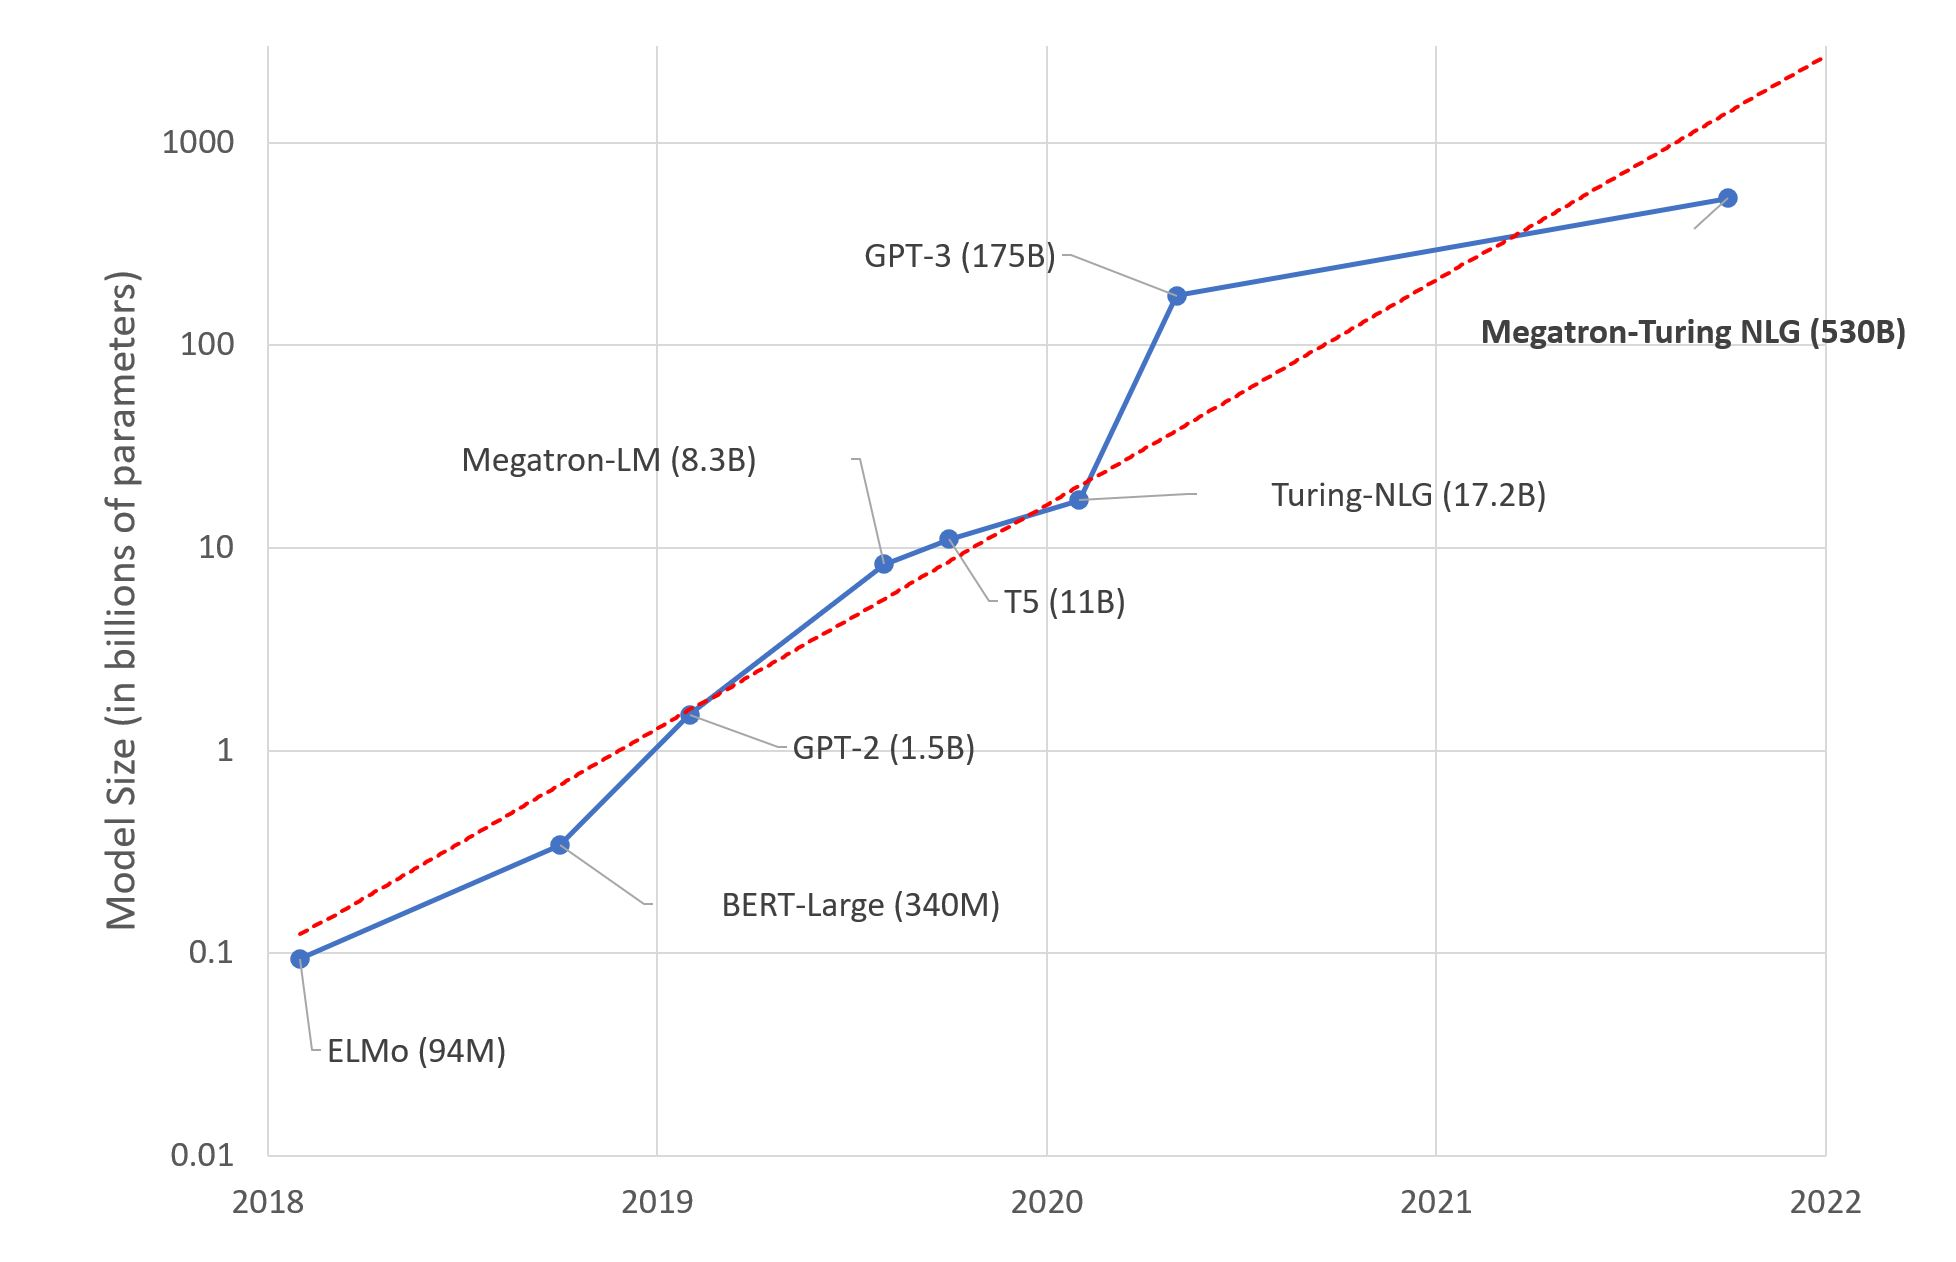
\includegraphics[width=\textwidth]{model_sizes}
    \caption{Model Sizes (2018--2021)~\cite{model_sizes}}
    \label{fig:model_sizes}
\end{figure}

However, despite their state-of-the-art performance, the inner workings of these models are not yet fully understood and these models are still considered opaque or \emph{black-box}~\cite{lei-etal-2016-rationalizing}, which is a problem for their adoption in critical applications, such as healthcare or finance 
where decisions need to be explainable and interpretable. 

The objective of this thesis is to explore the attention patterns and neural activations in Transformer architectures for sequence classification, more specifically, in context-free grammars.
This work is based on the hypothesis that the attention patterns and neural activations in these models can be used to explain the decisions made by the model, and that these explanations can be used to improve the model's performance and interpretability.